\chapter{Analysis of Security tools for the pipeline}
\label{chap:Tools}
\section{Introduction}
This chapter presents an introduction to the selected tools for this thesis and provides a description of their features. Additionally, the group will explain their reasoning behind selecting each of the different tools and look at the pros and cons of each. 


%\section{Snyk}
%Snyk\footnote{https://snyk.io/} is a comprehensive developer security platform that helps secure code, dependencies, containers, and infrastructure as code. It provides thorough scans of the code and alerts the user to any vulnerabilities. Beyond just checking the code, Snyk also examines installed dependencies, Docker containers, infrastructure as code, and more. This platform supports a wide range of programming languages and includes plugins compatible with various %\acrlong{ide}s.\cite{snyk1}

%\subsection{Why We Chose Snyk}
%The group decided on using Snyk because it is a well-known testing tool. It also has a reputation for being reliable, and user-friendly while it offers comprehensive security coverage. It also has a strong track record for quickly detecting vulnerabilities and alerting the users, which the group found %quite interesting and wanted to test further. \cite{snyk3}

\section{OWASP ZAP}
OWASP Zed Attack Proxy (ZAP)\footnote{https://www.zaproxy.org/} is an open-source web application security scanner. It is free and is maintained by volunteers across the world under the Open Web Application Security Project (OWASP). ZAP is a DAST tool and is designed to test web application security. The tool offers functionality for a wide range of people - from developers to experienced testers. It is available in versions that are compatible with major operating systems, as well as Docker, which means that users are not limited to a specific operating system when using the tool.\cite{owaspZAP}

\subsection{Why OWASP ZAP was chosen}
When the group started the research on different \acrshort{sast}, \acrshort{dast} and \acrshort{sca} tools, one of the \acrshort{dast} tools that were rapidly mentioned was OWASP ZAP - which claims to be the world's most widely used web app scanner. 
The group then discovered during research that there were some advantages to OWASP ZAP, one being easy to use and set up. Since ZAP is intended for use by people of diverse skill levels, the group thought it would be a beneficial tool because of minimal expertise with penetration testing. Another advantage is that OWASP ZAP is a free open-source tool, which makes it possible to try all functionality the software has to offer without any costs. OWASP ZAP is used when building pipelines in AWS and was easy to implement in AWS. These are some of the reasons why the group decided to use this tool. 

\subsubsection{Pros and cons}
These pros and cons are a combination of the personal experiences and information found during research.\cite{prosconsZAP}
\begin{table}[H]
    \centering
    \begin{threeparttable}
        \begin{tabular}{|c|p{6cm}|p{6cm}|}
            \hline
             & \textbf{Pros} & \textbf{Cons} \\
            \hline
            \textbf{OWASP ZAP} &
            \begin{itemize}
                \item [-]Open Source
                \item [-]Easy to configure with AWS
                \item [-] Free for both personal and commercial use
                \item [-]There are multiple application security testing approaches available that can help discover potential vulnerabilities
            \end{itemize}
            & 
            \begin{itemize}
                \item [-] Since it's open source, it may lack security\tnote{*}
                \item [-] The documentation could be improved and is, for some, difficult to understand
                \item [-]Compared to other tools, the automated scanning features are restricted
            \end{itemize}
            \\
            \hline
        \end{tabular}
        \begin{tablenotes}
            \item[*] There is a lot of debate around this topic,  with some claiming that open-source software is highly secure and others claiming that it can create risks. A list of advantages and disadvantages can be found at the following website: \href{https://cybersecuritynews.com/pros-and-cons-of-using-open-source-software/}{pros and cons website}
            \caption{Pros and cons of OWASP ZAP}
        \end{tablenotes}
    \end{threeparttable}
\end{table}


\section{Github Security Tools}
\subsection{Why tools integrated in GitHub was chosen}
Initially, the plan for the thesis  was to explore third-party tools, such as Snyk and Mend,  that could be integrated in Github and AWS and do an analysis of these. Nonetheless, a lecturer at NTNU Gjøvik suggested that the group could look closer into the in-built tools in GitHub and aws that perform \acrshort{sast}, \acrshort{dast} and \acrshort{sca} tests. The lecturer pointed out that examining third-party tools, such as Snyk, wouldn't be that intriguing since the third-party tools could already be considered up-to-date and reliable. On the other hand however, it could be interesting  to look into already in-built tools in AWS and Github and analyze these instead of implementing third-party tools. The reason behind the suggestion was that it could be useful to investigate tools that are already integrated and make a secure pipeline with these rather than look at state-of-the-art third-party tools. 

\subsection{Dependabot}
Dependabot is an in-built GitHub tool that helps developers keep their project dependencies up-to-date. A dependency can be considered a piece of code or software that the project that's being worked on needs and relies on. For example, the project might use a library or package that someone else has written, then this library/package can be considered a dependency of the project. 

Dependencies can be updated over time as new versions are released. Therefore, it is crucial that developers keep the dependencies up to date to ensure that the project stays secure. However, keeping track of all updates that come and manually running these updates can be frustrating since it can be rather time-consuming and error-prone. Dependabot automates the process of checking for new versions of the dependencies used in the code and then creates a pull request to update them. The user can then review the updates and see if it is necessary to do any changes or not. 
Dependabot can also automatically resolve any conflict that may arise when updating dependencies and can even open up separate pull requests for separate dependency updates.  \cite{GithubDependabot2}

Dependabot uses the "GitHub Advisory Database" to check for vulnerable data. This database covers a lot of public vulnerabilities and it uses multiple sources, like \acrlong{cve}, \acrlong{nvd}, and several others. \cite{GithubDependabot1}

%\subsection{Why Dependabot was chosen}
%Dependabot was chosen to gain a better understanding of tools that are already integrated into GitHub instead of implementing third-party tools for the different application security tests. This was to evaluate the necessity of a third-party tool, given that GitHub already offers tools that are widely used by developers. The group found it reasonable to assume that GitHub provides sufficient tools making it unnecessary to implement a third-party tool, which is the reason why the group decided to %test this theory. 
\subsubsection{Pros and cons}
These pros and cons are a combination of the personal experiences and information found during research. \cite{prosconsdependabot} 

\begin{table}[H]
\centering
\begin{tabular}{|c|p{6cm}|p{6cm}|}
\hline
 & \textbf{Pros} & \textbf{Cons} \\
\hline
\textbf{Dependabot} & 
- Automates dependency updates, saving time and reducing manual errors \newline
- Supports a wide range of languages and package managers \newline
- Provides detailed changelogs and release notes \newline
- Integrates with various development tools and services &
- Dependabot sends a notification for every update which can quickly 
  become overwhelming. \newline
- Can create merge conflicts with other changes \newline
- Its automatic scans can generate many false positives which can be 
  time-consuming. \\
\hline
\end{tabular}
\caption{Pros and Cons of Dependabot}
\label{tab:dependabot}
\end{table}

\subsection{Code Scanner}
GitHub has an in-built code scanning tool called CodeQL that allows the users to analyze the code that is in the GitHub repository to find vulnerabilities and errors in the code. The results of these analyzes are shown as code-scanning alerts in GitHub.This feature helps identify existing issues but also prevents new ones from being introduced. \cite{CodeQL1}

CodeQL can be scheduled so that it runs on chosen days or occurrences of events. Rather than scanning each branch individually, it is possible to set up a trigger that will initiate the code scan only when the code is pushed to the main branch or when a pull request is made to the main branch. This helps to reduce the amount of time and resources required to perform the scans. Also, it minimizes the risk of vulnerabilities or errors being introduced into the production environment.

Any issues found during the scanning process are displayed as alerts within the repository. This means that developers can divide the different fixes easily between members of the team.  Once a user fixes the code that triggered the alert, it is automatically closed. Additionally, users can monitor the results of code scanning across their repositories or organization using web-hooks and the code scanning API. 
\cite{GithubCodeScanning}

\begin{comment}
    CodeQL and Dependabot have together detected 101 vulnerabilities. This is the exact amount of vulnerabilities that were "...intentionally planted in the application..." \cite{owaspJuiceShop}.
\end{comment}

\subsubsection{Pros and cons}
\begin{table}[H]
\centering
\begin{tabular}{|c|p{6cm}|p{6cm}|}
\hline
 & \textbf{Pros} & \textbf{Cons} \\
\hline
\textbf{Code Scanning} & 
- Triggers: Teams can decide when they want the scanning to be triggered. This is usually when an event occurs, such ass pull requests.  \newline
- Configure the scan to suit the project: The scan can be configured so that it tailors the 
  different needs. \newline
- Auto-build: When code scanning runs, it automatically uploads the vulnerabilities it found to the repository's security tab. &
- CodeQL isn't always as well-suited for certain types of projects. \newline
- CodeQL's precision can depend on the quality of the code\newline
- CodeQL only supports a smaller set of languages \newline
- May require configuration and customization to fit project needs \\
\hline
\end{tabular}
\caption{Pros and Cons of Code Scanning}
\label{tab: Code Scanning}
\end{table}


\subsection{Secret Scanner}
GitHub's Secret scanner is an in-built tool that analyzes the code on all branches to see if there are any secrets within the code. Such secrets can be tokens or private keys. This is the case for archived repositories as well. To authenticate with an external service, developers may require a token or a private key, which can be issued by a service provider. However, if these secrets get added to the repository, anyone with read access can use these to their advantage and get access to the external service. Therefore it is highly recommended that such secrets are stored outside the repository. However, secret scanning is created to alert about such secrets when detected. Developers can get the
security scanner in two forms\cite{GithubSecretScanning}: 
\begin{itemize}
    \item \textbf{Secret Scanning alerts for users}\\
GitHub's security scanning for users is intended for organizations that have licensed GitHub Advanced Security and it provides the ability to enable and configure scanning for private and internal repositories. This feature allows users to define their own custom pattern-matching rules to identify secrets in code and will report any matches in the security tab of the repository for review by the organization. 

Overall, security scanning for users allows organizations to define their own custom rules and enables scanning for private and internal repositories.

\item \textbf{Secret Scanning alerts for partners}\\
This feature can be enabled for teams that use the GitHub Enterprise Cloud and have a license for GitHub Advanced Security. This means that, to access this form the repositories have to be owned by an organization that has a license to GitHub Advanced Security. It is not available for repositories that are owned by individuals. 

When Secret Scanning for users is activated, GitHub will search for secrets used by various service providers. If any supported secrets are detected, a secret scanning alert will be generated by GitHub Enterprise Cloud.
GitHub's Secret scanning for partners is intended for third-party service providers who have partnered with GitHub to provide pre-defined pattern-matching for identifying secrets in code. This feature is available for all public repositories and will report any matches of these predefined patterns directly to the relevant partner for their review and action. 

Overall, secret scanning for partners focuses on providing predefined pattern-matching rules to third-party service providers. 
\end{itemize}
\subsubsection{Pros and cons}


\section{Amazon Web Services Tools}
\begin{comment}
\subsection{AWS Lambda}
According to \acrshort{aws},  Lambda is considered a serverless compute server and is created for developers to be able to run code in the cloud without having the need to set up any servers.\cite{AWSLamda} It is an on-demand service, which means that developers only pay for what they use. Lambda can be integrated with many different services in the \acrshort{aws} cloud, which means that developers can build rather complex backends and pipelines. 

\acrshort{aws} Lambda is what is called an "event-driven" service, which means that it executes code as a response to different events created. Such events can be a lot of things, it can for example be events that have been generated from other \acrshort{aws} services like \acrshort{aws} based data processing pipelines or HTTP endpoints. 

Lambda supports a large amount of different programming languages, such as Python, JavaScript and Ruby etc. However, it also allows developers to create custom runtimes for languages that are not necessarily supported. 
\end{comment}

\subsection{AWS CodePipeline}
In short \acrshort{aws} CodePipeline is a "\textit{...fully managed continuous delivery service that helps you automate your release pipeline. It allows users to build, test, and deploy code into a test production environment...}"
\cite{AWSCodePipeline}

CodePipeline automates the entire \gls{Pipeline}, including the build, test, and deploy phases, and triggers these processes whenever changes are detected in the repository. When a developer pushes changes to the repository, CodePipeline automatically detects the changes and initiates the process by building them. If any tests are configured, CodePipeline also runs these tests.\cite{AWSCodePipeline1}
\begin{figure}[H]
    \centering
    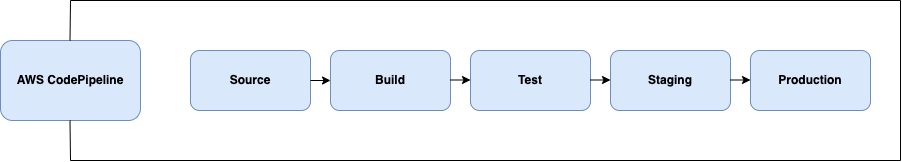
\includegraphics[scale=0.4]{Images/CodePipeline.png}
    \caption{AWS CodePipeline process}Adapted from: \cite{AWSCodePipeline2}
    \label{fig: AWS CodePipeline Process}
\end{figure}

\subsection{AWS CodeBuild }
AWS CodeBuild can be described as a "\textit{...fully managed continuous integration service that compiles source code, runs tests, and produces ready-to-deploy software packages.}"
\cite{AWSCodeBuild}
What AWS CodeBuild does is that it downloads the source code provided to it into a build environment and then uses a \Gls{buildspec} which defines how the built project should be executed\cite{AWSCodeBuild1}
\begin{figure}[H]
    \centering
    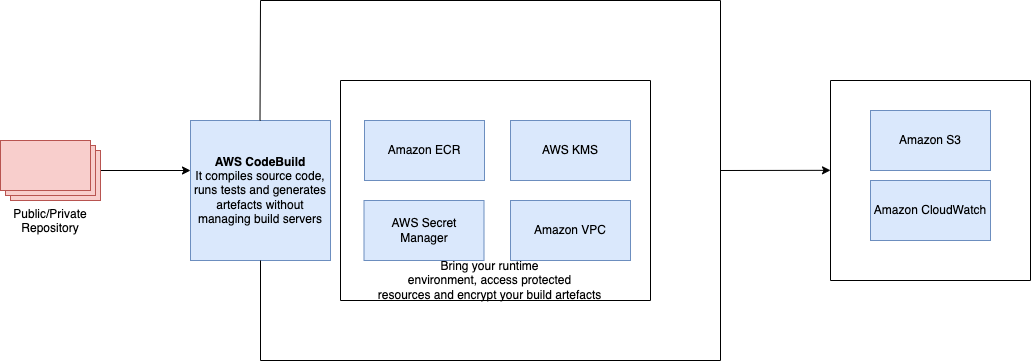
\includegraphics[scale=0.4]{Images/CodeBuild.png}
    \caption{AWS CodeBuild process}\cite{AWSCodeBuild}
    \label{fig: AWS CodeBuild Process}
\end{figure}

\subsection{AWS CodeDeploy}
\acrshort{aws} CodeDeploy is numbered as "\textit{...a fully managed deployment service that automates software deployments to various compute services, such as Amazon Elastic Compute Cloud (EC2), AWS Lambda and more[...]}"\cite{AWSCodeDeploy}.
\acrshort{aws} CodeDeploy helps developers avoid downtime during deployment. It also handles the updating phase of the applications. 

CodeDeploy can deploy code that runs on a server and is stored in for example GitHub repositories or in a \acrshort{aws} S3 Bucket. In order to use CodeDeploy, developers are not required to make any adjustments to their existing code. \cite{CodeDeploy1}

\begin{figure}[H]
    \centering
    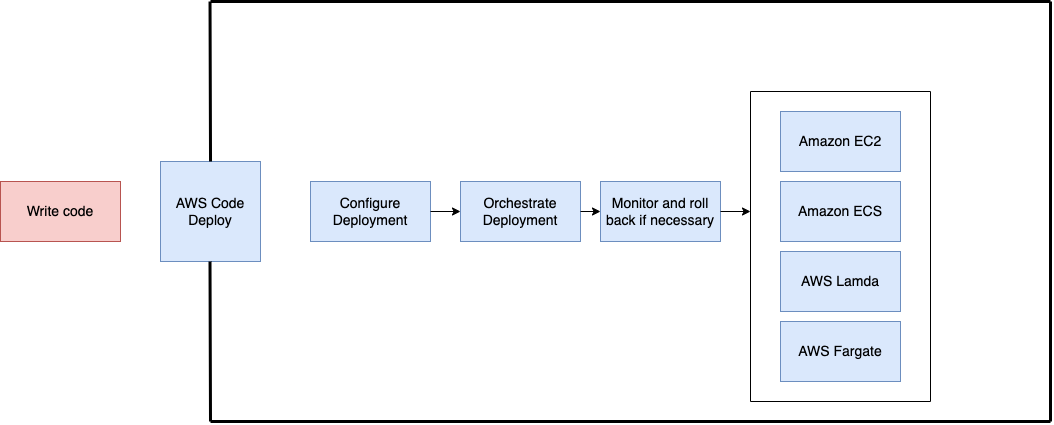
\includegraphics[scale=0.4]{Images/AWSCodeDeploy.png}
    \caption{AWS CodeDeploy process} Adapted from: \cite{CodeDeploy1}
    \label{fig:AWS CodeDeploy Process}
\end{figure}


\subsection{AWS S3 buckets}
\acrshort{aws} S3 buckets are simple storage resources that are known to be cloud-based. Amazon S3 buckets are designed to provide users with scalable, durable, and highly available storage which can be used to store different types of data. Such data can be documents, artifacts, source code, and so on. An S3 bucket can be considered a container that stores different objects. \cite{S3Bucket}

\subsection{AWS EC2}
\acrlong{ec2} offers a \gls{compute platform}, with virtual computing environments, also known as instances. \acrlong{ec2} offers a wide range of instance types to meet different computing needs. These instances come with preconfigured templates called \acrlong{amis} that contain the necessary software and operating system to run the server. Users can choose from various configurations of CPU, memory, storage, and networking capacity for their instances, known as instance types.\cite{awsec2}

\subsection{AWS CodeStar Connections}
\acrshort{aws} CodeStar Connection is a tool from \acrshort{aws} that enables users to connect to third-party repositories for \acrshort{aws} to retrieve their code. This tool can be configured to a specific branch, so when new code is pushed or merged, CodeStar Connection will fetch the code from the repository and place it in an S3 bucket.\cite{AWSCodeStarConnections}